\chapter[Introduction]{Introduction}\label{chap-intro}

%%%%%%%%%%%%%%%%%%%%%%%%%%%%%%%%%%%%%%
\section{Background}
%%%%%%%%%%%%%%%%%%%%%%%%%%%%%%%%%%%%%%

It is a good idea to discuss the structure of the report with your supervisor rather early in your writing.

%%%%%%%%%%%%%%%%%%%%%%%%%%%%%%%%%%%%%%
\section{Sample Table}

As a recommendation, use regular paragraph text in the tables, bold headings and avoid vertical lines (see Table \ref{tab:margins}). 

\begin{table}
\centering
\caption{Text margins for A4.}\label{tab:margins}
\begin{tabular}{cc}
\hline
\textbf{margin} & \textbf{space} \\
\hline 
top &  3.0cm\\ 
bottom & 3.0cm \\ 
left (inside) & 2.5cm \\ 
right (outside) & 2.5cm \\ 
binding offset & 1.0cm \\ 
\hline 
\end{tabular} 
\end{table}

%%%%%%%%%%%%%%%%%%%%%%%%%%%%%%%%%%%%%%
\section{Sample Figure}

As a recommendation, use vector graphics in figures (Figure \ref{fig:vectorg}), rather than bitmaps (Figure \ref{fig:rasterg}). Text within figures usually looks better with sans-serif fonts.  I prefer to use \texttt{width} to adjust the width of figures and set sizes relative to the line width instead of using \texttt{scale}.

\begin{figure}
\centering
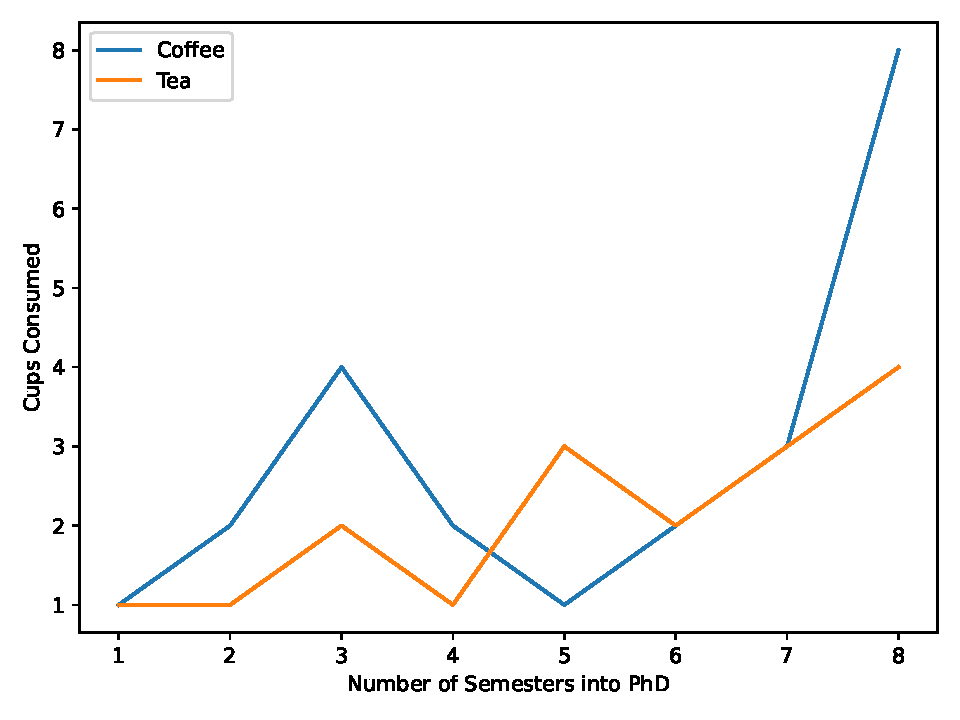
\includegraphics[width=1\linewidth]{Figures/Figure_1.pdf} 
\caption{A PDF vector graphics figure. Notice the numbering and placement of the caption. The caption text is indented 2.0cm from both left and right text margin.}\label{fig:vectorg}
\end{figure}

\begin{figure}
\centering
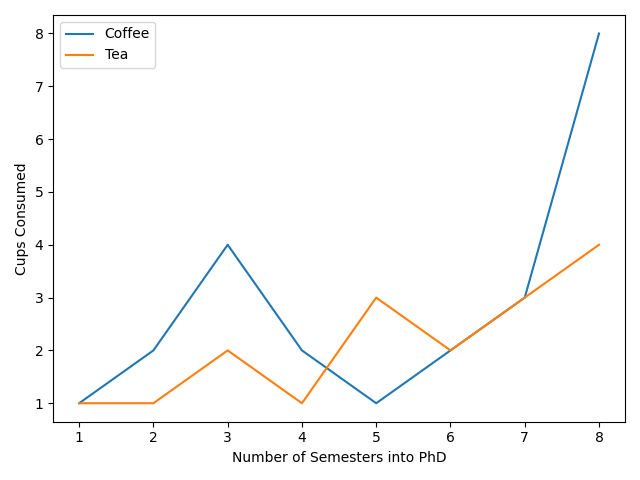
\includegraphics[width=1\linewidth]{Figures/Figure_1.png} 
\caption{A PNG bitmap figure. Notice the bad quality of such an image when scaling it. Sometimes bitmap images are unavoidable, such as for screen dumps.}\label{fig:rasterg}
\end{figure}

\begin{figure}
\centering
\begin{adjustbox}{
  addcode={\begin{minipage}{\width}}{
    \caption{You can use the adjustbox environment to rotate an image if you have trouble fitting it on a page.}\label{fig:rotated}
    \end{minipage}
  },rotate=90,center}
  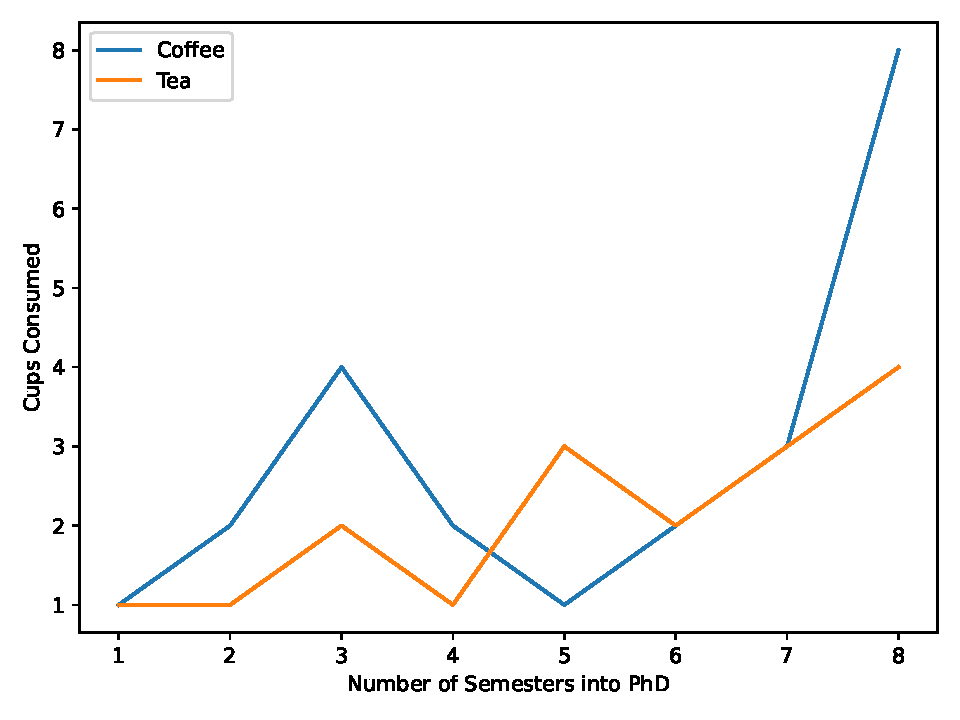
\includegraphics[width=1\linewidth]{Figures/Figure_1.pdf}
\end{adjustbox}
\end{figure}

\begin{figure}
\centering
\begin{subfigure}{0.45\textwidth}
  \centering
  \captionsetup{width=0.9\linewidth}
  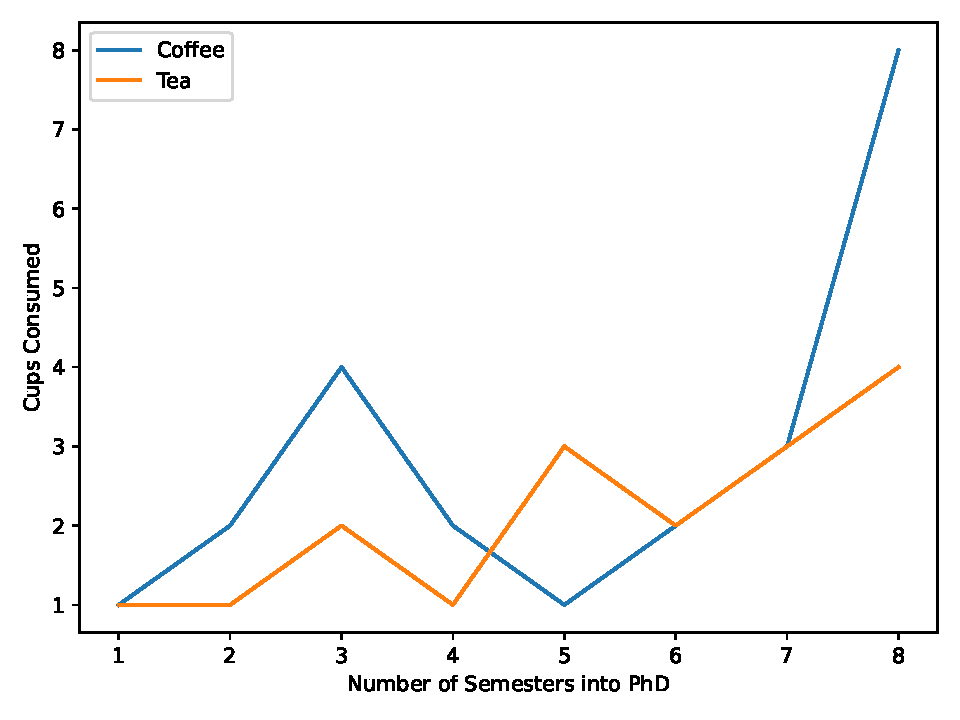
\includegraphics[width=1\linewidth]{Figures/Figure_1.pdf}
  \caption{This is a sub-caption.}
  \label{subfig:a}
\end{subfigure}
\begin{subfigure}{0.45\textwidth}
  \centering
  \captionsetup{width=0.9\linewidth}
  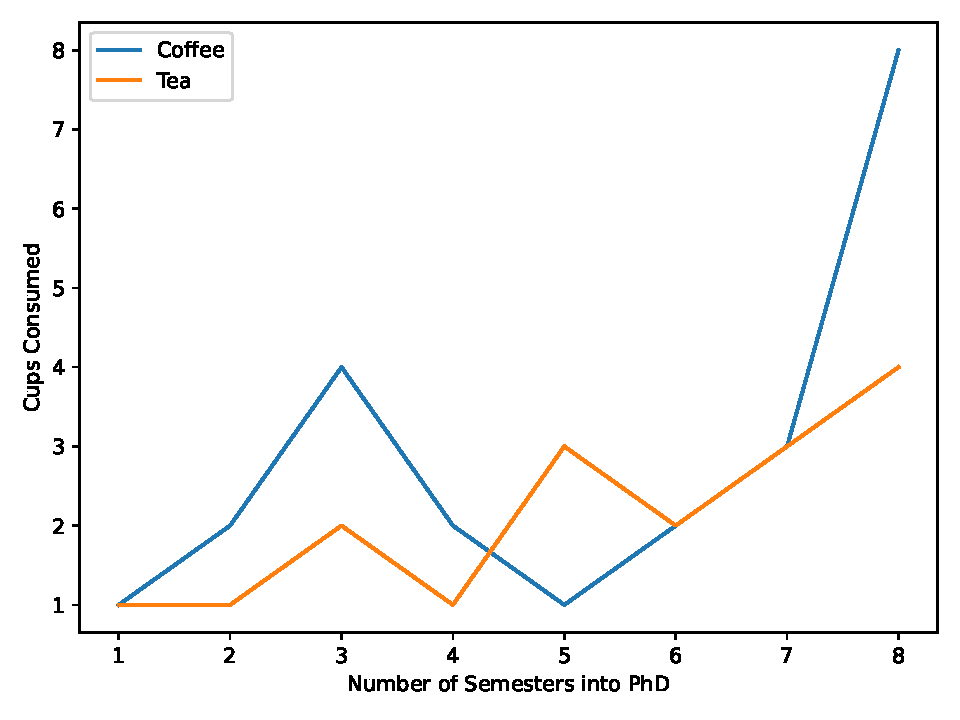
\includegraphics[width=1\linewidth]{Figures/Figure_1.pdf}
  \caption{This is another sub-caption.}
  \label{subfig:b}
\end{subfigure}
\caption{Caption for the entire figure.  I find the sub-figure captions look better if the width is set to 0.9.}
\label{fig:subfigs}
\end{figure}

%%%%%%%%%%%%%%%%%%%%%%%%%%%%%%%%%%%%%%
\section{Sample Equation}

You are free to use in-text equations and formulae, usually in \textit{italic serif} font. For instance: $S = \sum_i a_i$. We recommend using numbered equations (e.g. Equation \ref{eqn:emc1} when you do need to refer to the specific equations:

\begin{equation}
E = \int_0^{\delta} P(t) dt \quad \longleftrightarrow \quad E = m c^2
\label{eqn:emc1}
\end{equation} 

%%%%%%%%%%%%%%%%%%%%%%%%%%%%%%%%%%%%%%
\section{Sample Algorithm}

I like to use the Algorithm2e package for pseudocode like in the ACM journal template (e.g. Algorithm~\ref{alg:binary_search}).

\begin{algorithm}
\caption{Find the index of an element in an ordered list.}
\label{alg:binary_search}
\KwIn{Ordered list $L = \{ L_0 \dots L_n \}$, and a value $v$}
\KwOut{Index $m$ of value $v$ in $L$}
$l = 0$;
$r = n - 1$;
\While{$L_m \neq v$}{
  $m = \lfloor (l + r) / 2 \rfloor$;
  \uIf{$L_m < v$}{
    $l = m + 1$;
  }
  \uElseIf{$L_m > v$}{
    $r = m - 1$;
  }
  \uElse{
    \Return $m$;
  }
}
\Return $\emptyset$;
\end{algorithm}

%%%%%%%%%%%%%%%%%%%%%%%%%%%%%%%%%%%%%%
\section{Theorems, Lemmas, and Proofs}

\begin{theorem}
    Theorems are defined like this.
\end{theorem}
\begin{proof}
    The proof environment should immediately follow.
\end{proof}

\begin{lemma}
    Lemmas can be defined in a similar manner.
\end{lemma}
\begin{proof}
    This is the proof associated with the lemma.
\end{proof}
